\documentclass[10pt, xcolor=table]{beamer}
\usepackage{inputenc}
\usepackage{graphicx}
\usepackage {mathtools}
\usetheme{CambridgeUS}
\usecolortheme{dolphin}
\usepackage{booktabs}
\usepackage{lscape}
\usepackage{caption}
\usepackage{tikz}
\usepackage{subcaption}
\usepackage{multicol}
\usepackage{xcolor}
\usepackage{pgfplots}
\usepackage{bm}
\usepackage{multicol}
\usepackage{adjustbox}
\usepackage{multicol}
\usepackage{cleveref}
\usepackage{tcolorbox}
\usepackage{changepage}
\usepackage{pifont}    % For more symbols like dingbats
\usepackage{blindtext}
\usepackage{array}
\usepackage{diagbox}

\newcommand\dc[1]{\textcolor{blue}{#1}}
\setcounter{tocdepth}{3}
\pgfplotsset{compat=1.16}
%\usetikzlibrary{external}
%\tikzexternalize[prefix=images/]

\newlength\figureheight
\newlength\figurewidth

\definecolor{myNewColorA}{HTML}{952748}
\definecolor{myNewColorB}{HTML}{ffe7ee} 
\definecolor{myNewColorC}{HTML}{c86666}
\definecolor{myNewColorD}{HTML}{eaa1a1} 
\definecolor{background_color}{HTML}{000000}

\setbeamercolor*{palette primary}{bg=myNewColorC}
\setbeamercolor*{palette secondary}{bg=myNewColorB, fg=black}
\setbeamercolor*{palette tertiary}{bg=myNewColorA, fg=white}
\setbeamercolor*{titlelike}{fg=myNewColorA}
\setbeamercolor*{title}{bg=myNewColorA, fg=white}
\setbeamercolor*{item}{fg=myNewColorB}
\setbeamercolor*{caption name}{fg=myNewColorA}

% For NN graph

\usepackage{listofitems} % for \readlist to create arrays
\usetikzlibrary{arrows.meta} % for arrow size
\usepackage[outline]{contour} % glow around text
\contourlength{1.4pt}


% STYLES
\tikzset{
	>=latex, % for default LaTeX arrow head
	node/.style={thick,circle,draw=myblue,minimum size=22,inner sep=0.5,outer sep=0.6},
	node in/.style={node,green!20!black,draw=mygreen!30!black,fill=mygreen!25},
	node hidden/.style={node,blue!20!black,draw=myblue!30!black,fill=myblue!20},
	node convol/.style={node,orange!20!black,draw=myorange!30!black,fill=myorange!20},
	node out/.style={node,red!20!black,draw=myred!30!black,fill=myred!20},
	connect/.style={thick,mydarkblue}, %,line cap=round
	connect arrow/.style={-{Latex[length=4,width=3.5]},thick,mydarkblue,shorten <=0.5,shorten >=1},
	node 1/.style={node in}, % node styles, numbered for easy mapping with \nstyle
	node 2/.style={node hidden},
	node 3/.style={node out}
}
\def\nstyle{int(\lay<\Nnodlen?min(2,\lay):3)} % map layer number onto 1, 2, or 3

\usefonttheme{professionalfonts}



%\usepackage[round]{natbib} % or use 'authoryear' if you prefer
%\usepackage{natbib}
\usepackage{hyperref}
%------------------------------------------------------------
\titlegraphic{
	\begin{figure}
		\centering
		\begin{subfigure}[l]{0.45\textwidth}
			\centering
			
\includegraphics[width=2.5cm,height=1.5cm]{./Logo_U.T.P.png}
		\end{subfigure}
		\hfill
		\begin{subfigure}[r]{0.45\textwidth}
			\centering
			
\includegraphics[width=2.5cm,height=2.5cm]{./logo-maestria-scaled.jpg}
		\end{subfigure}
	\end{figure}
}

\setbeamerfont{title}{size=\Large\bfseries}
\setbeamerfont{subtitle}{size=\footnotesize}
\setbeamerfont{author}{size=\small}
\setbeamerfont{institute}{size=\footnotesize}

\title[Universidad Tecnológica de Pereira]{Data-Driven Models for Identifying Mental Disorders in Students and Enhancing Therapy Scheduling}



\author[Julián David Pastrana-Cortés]{%
	\texorpdfstring{
		\begin{tabular}{c}
			M.Sc. Julián David Pastrana-Cortés \\[1.5mm]
			%			\textbf{Director}: Álvaro Angel Orozco-Gutiérrez \\[1.5mm]
			%			\textbf{Co-director}: David Augusto Cardenas-Peña
		\end{tabular}
	}{Julián David Pastrana-Cortés\vspace{-20pt}}
}

\institute[Automatics]{Automatics Research Group\vspace{-15pt}}
%\date{\today\vspace{-15pt}}

\AtBeginSection[]{
	\begin{frame}
		\vfill
		\centering
		\begin{beamercolorbox}[sep=8pt,center,shadow=true,rounded=true]{title}
			\usebeamerfont{title}\insertsectionhead\par%
		\end{beamercolorbox}
		\vfill
	\end{frame}
}

\usepackage{ragged2e} % For \justifying command
\usepackage{lipsum} % Only for demo text

\addtobeamertemplate{block begin}{}{\justifying} 
%\addtobeamertemplate{itemize begin}{}{\justifying} 


%------------------------------------------------------------

\usepackage{etoolbox}

\apptocmd{\frame}{}{\justifying}{} 
\let\olditem\item
\renewcommand\item{\olditem\justifying}

\begin{document}
	
	\frame{\titlepage}

	
	
	\section*{Mental Disorders}
	
	\begin{frame}{Understanding Mental Disorders}
		A mental disorder refers to a significant disturbance in an individual's cognition, emotional regulation, or behavior.
		
		\begin{multicols}{2}
			
			\begin{figure}[t]
				\centering
				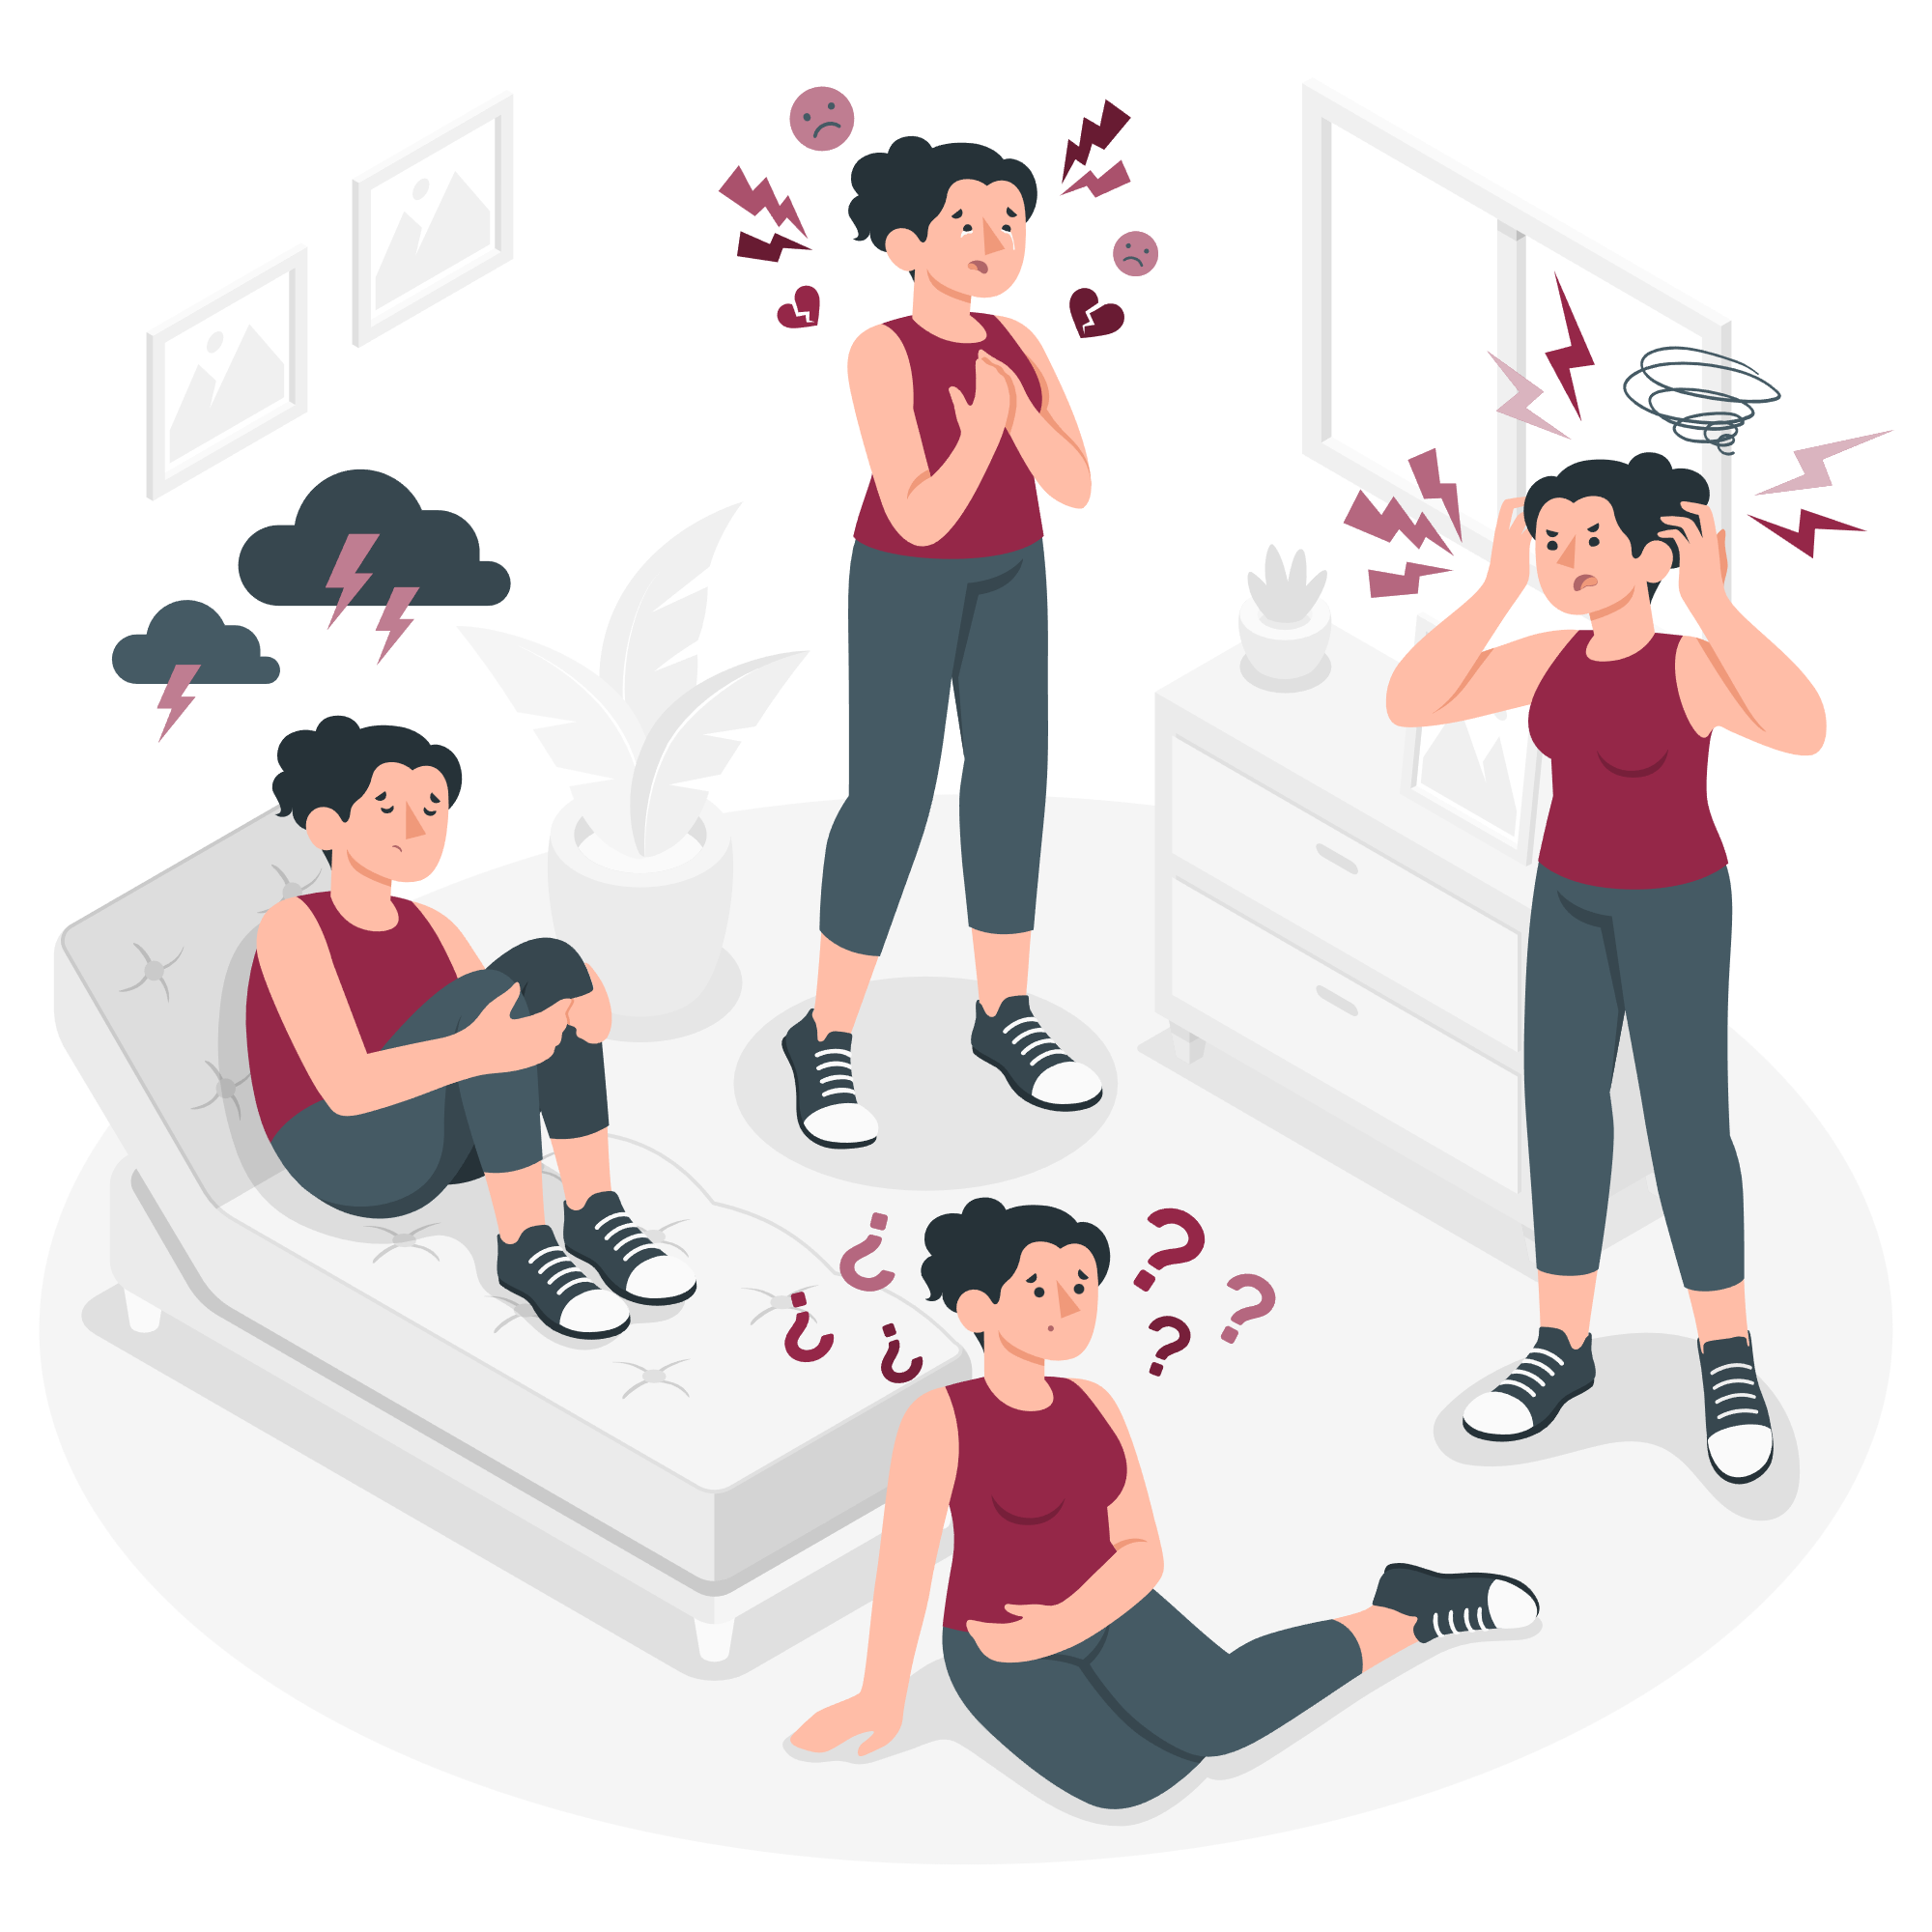
\includegraphics[width=0.8\linewidth]{./figures/mental_disorders.png}
			\end{figure}
			
			\columnbreak
			
			\vfill
			\begin{center}
				\begin{itemize}
					\item \textbf{Depression}: Persistent feelings of sadness and loss of interest.
					\item \textbf{Anxiety}: Excessive fear or worry, often irrational.
					\item \textbf{Impulsivity}: Acting without thought or consideration of consequences.
					\item \textbf{Hyperactivity}: Excessive movement, often interfering with daily activities.
				\end{itemize}
			\end{center}
			
			\vfill
			
		\end{multicols}
		
		Over 350 million individuals worldwide suffer from mental disorders \cite{DEHGHANBONARI2023100238}.
		
	\end{frame}
	
	
	\begin{frame}{Why Accurate Diagnosis Matters for Students?}
		\begin{columns}
			\begin{column}{0.5\textwidth}
				\begin{itemize}
					\item Mental health disorders can significantly impact students' academic and social lives \cite{HAMORI2023115139}.
					\item External factors, such as homesickness and family expectations, can intensify mental health issues \cite{DEHGHANBONARI2023100238}.
					\item Anxiety and depression, the most common mental health concerns among U.S. college students, have been on the rise \cite{https://doi.org/10.1002/jcad.12543}.
				\end{itemize}
			\end{column}
			\begin{column}{0.5\textwidth}
				\begin{figure}[t]
					\centering
					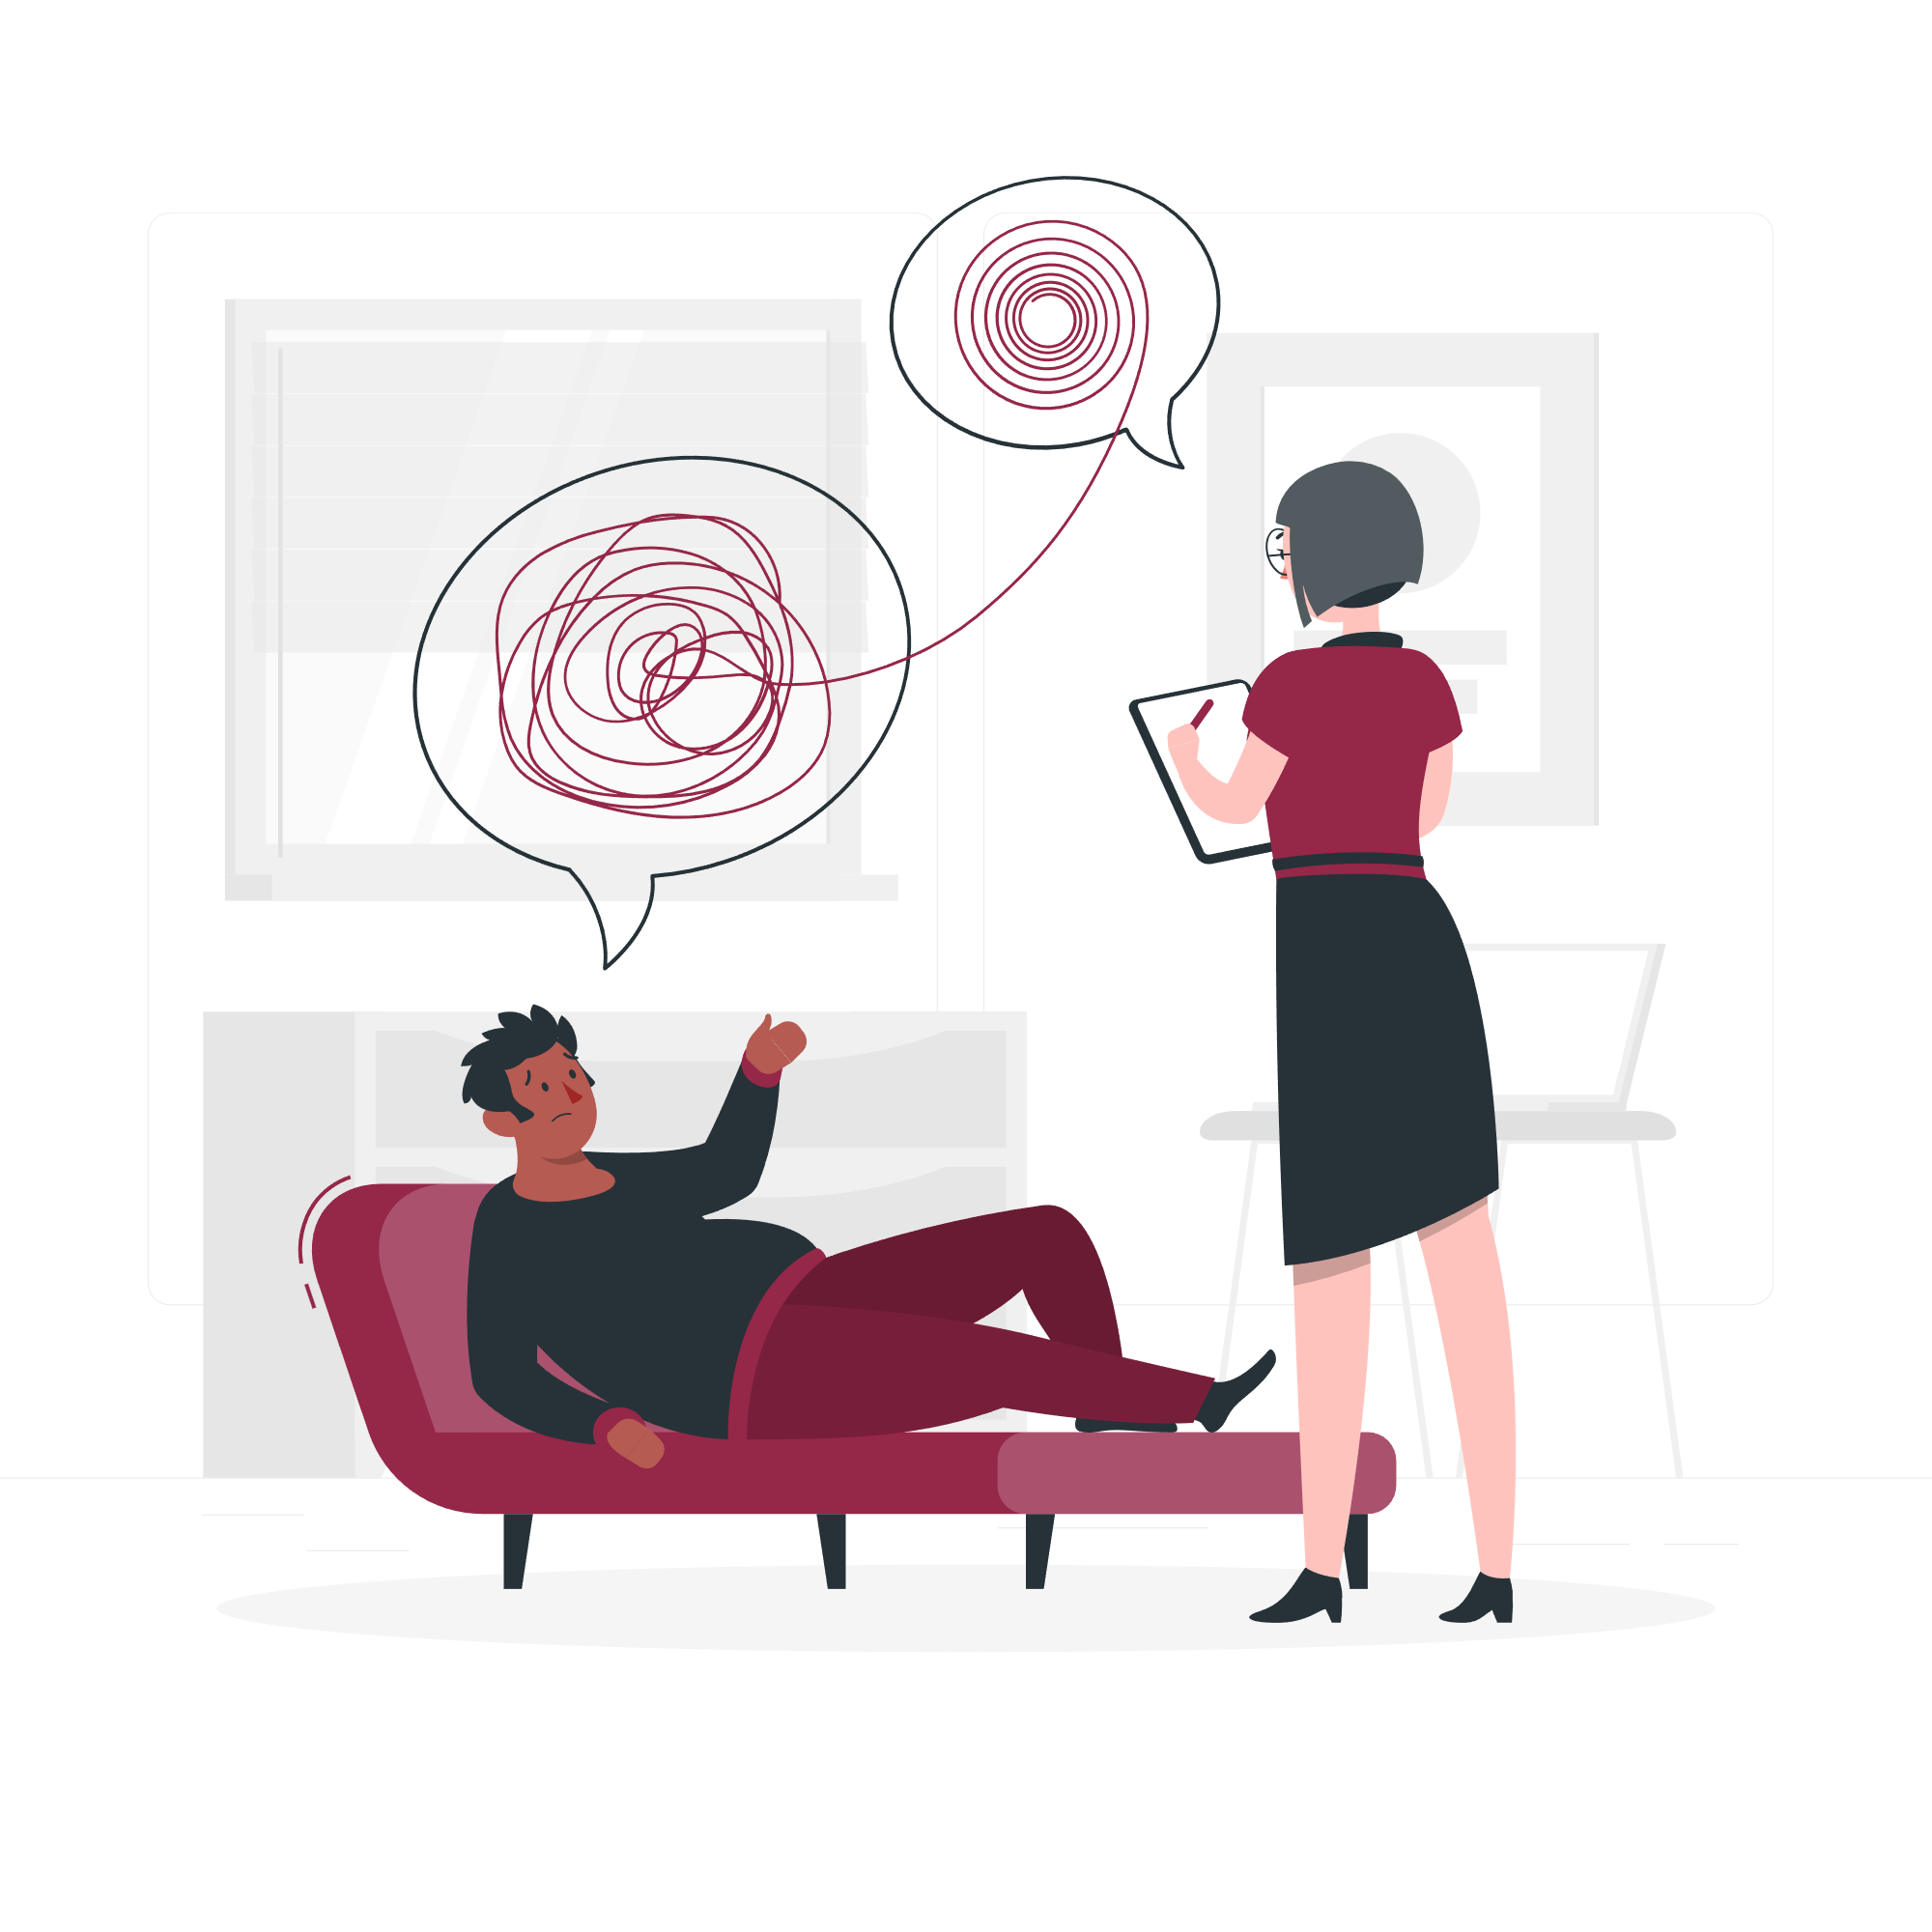
\includegraphics[width=\linewidth]{./figures/psychologist.png}
				\end{figure}
			\end{column}
		\end{columns}
	\end{frame}
	
\begin{frame}{Challenges}
	
	\begin{columns}
		% Column for the image
		\begin{column}{0.5\textwidth}
			\begin{figure}[t]
				\centering
				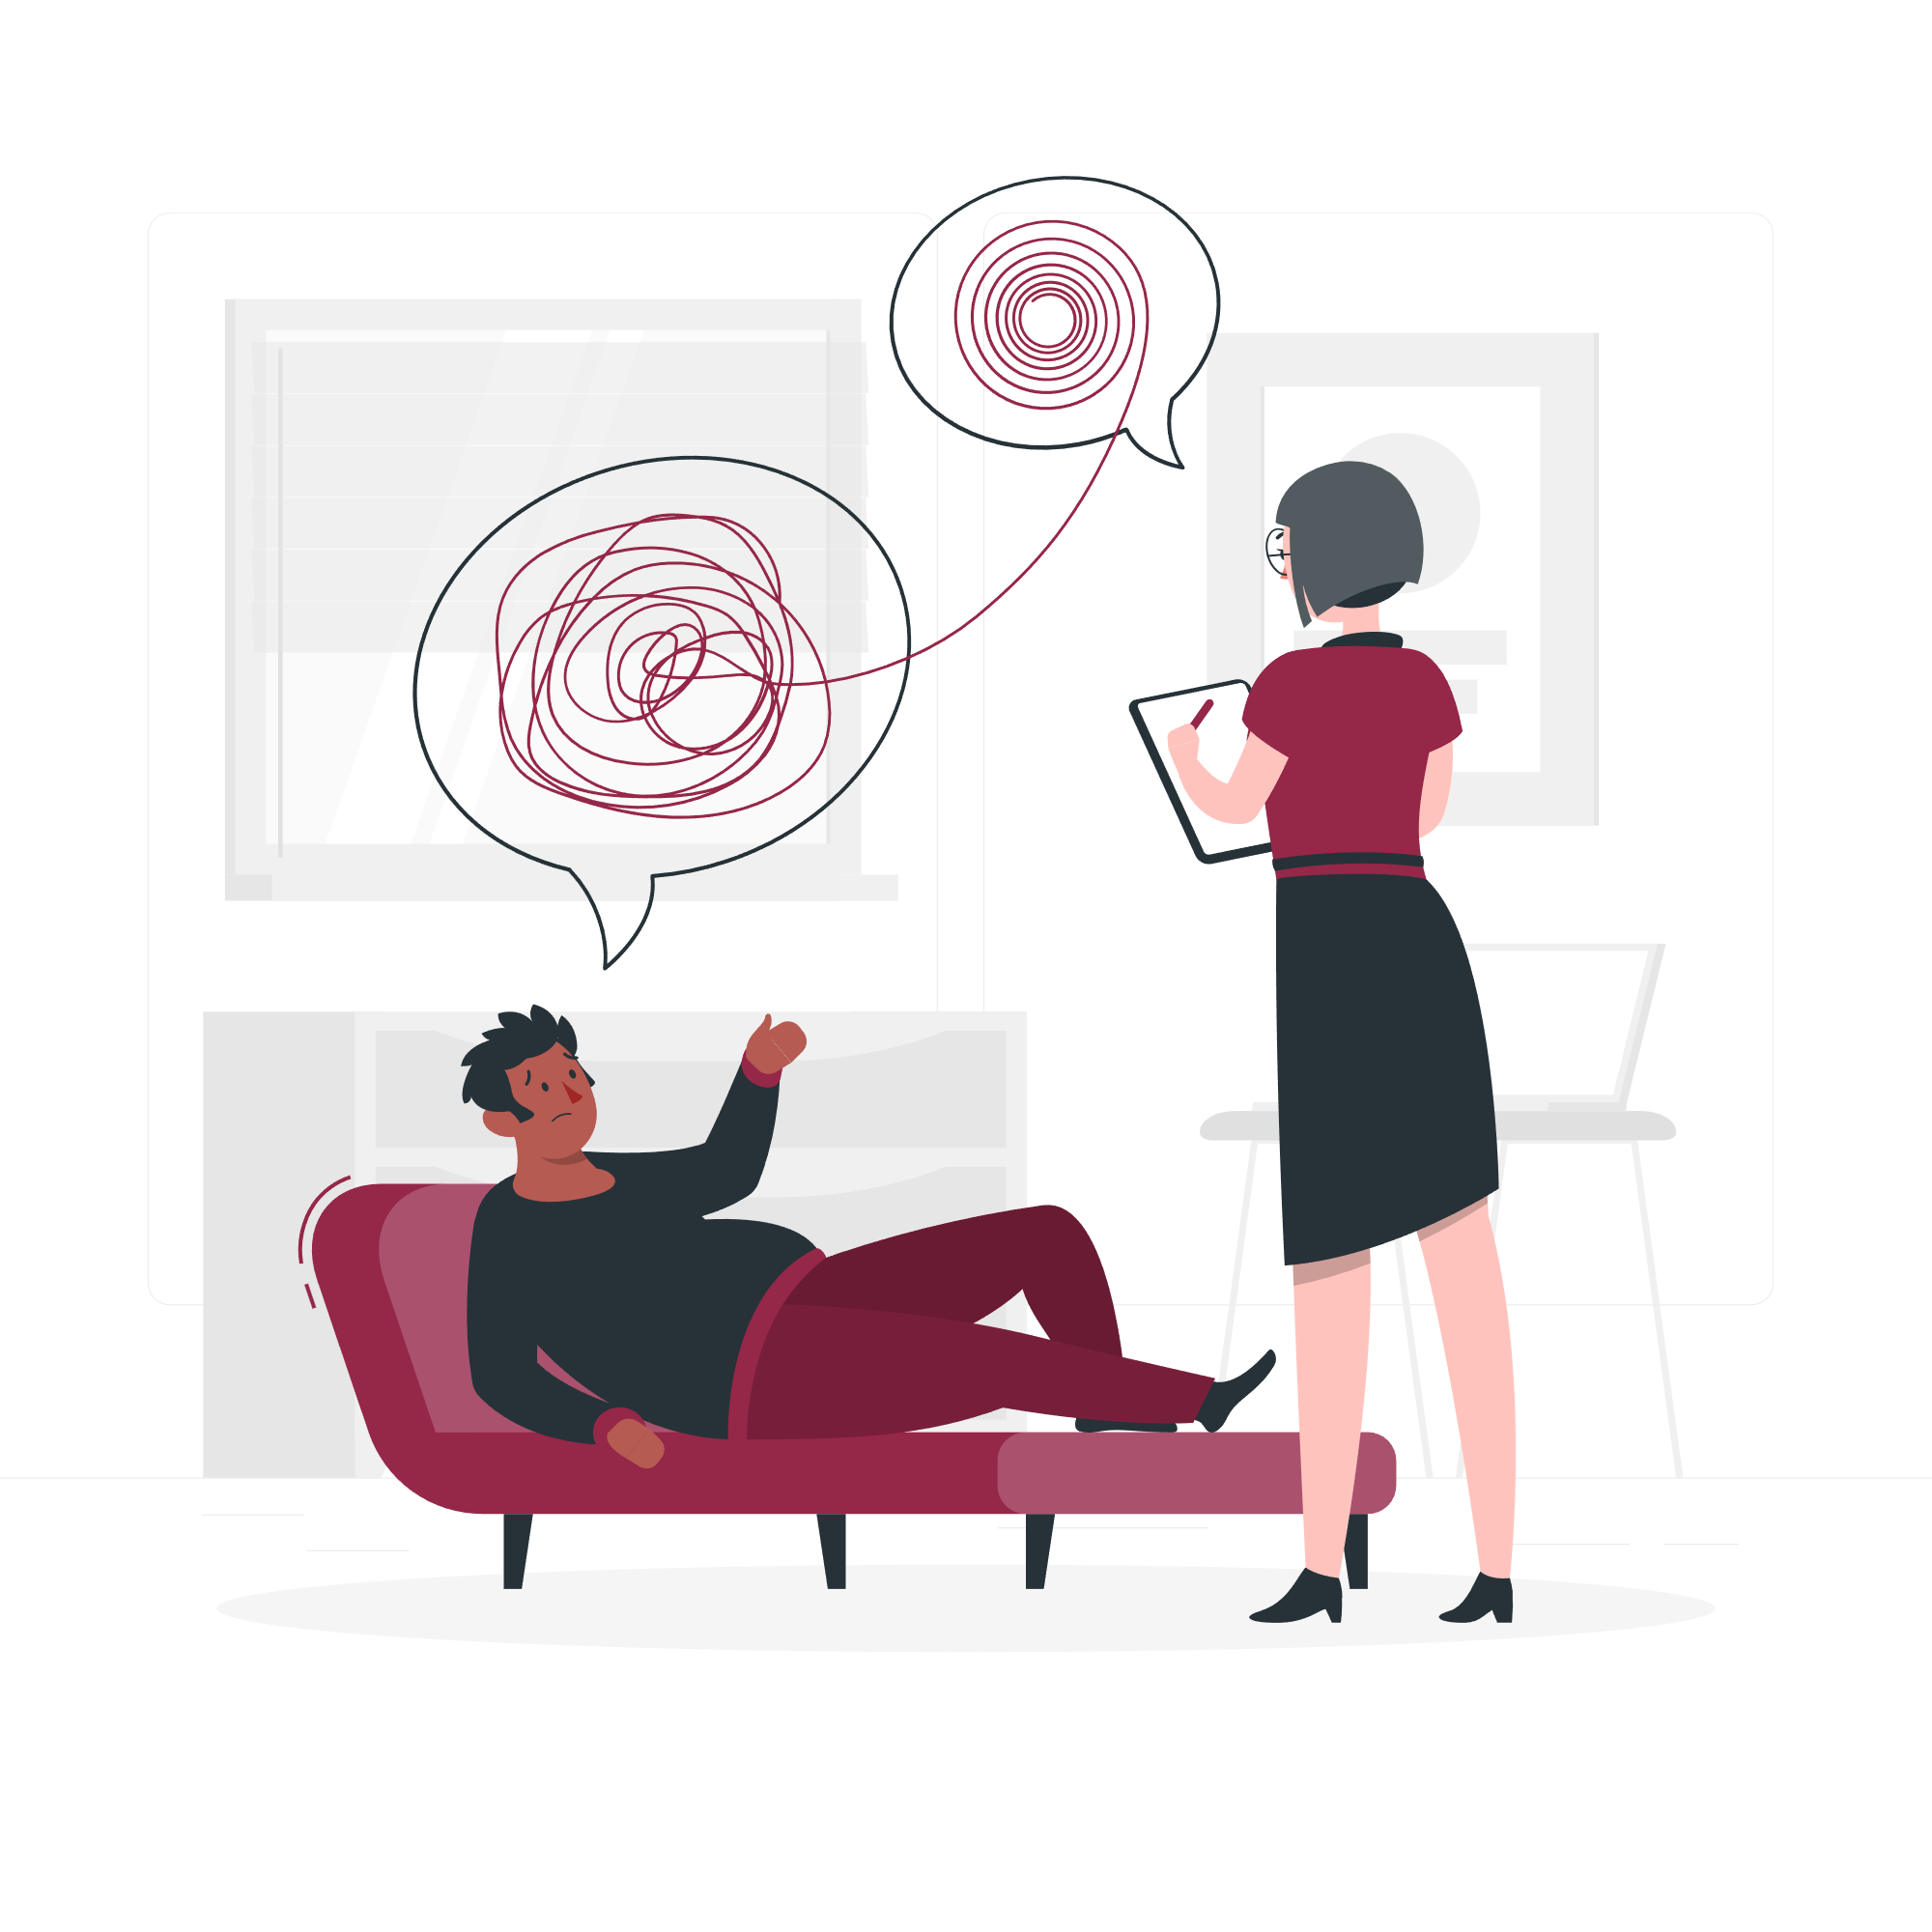
\includegraphics[width=\linewidth]{./figures/psychologist.png}
			\end{figure}
		\end{column}
		
		% Column for the text
		\begin{column}{0.5\textwidth}
			\begin{itemize}
				\item A severe shortage of trained mental health professionals and infrastructure persists in many parts of the world, especially in developing countries \cite{SHARMA2024e32548}.
				
				\item Accessible methods that can integrate seamlessly into patients’ daily lives are urgently needed \cite{NGUYEN20231458}.
				
				\item Reducing the burden associated with mental disorders requires prioritizing early prevention before problems arise. \cite{GRUMMITT2023200308}.
			\end{itemize}
		\end{column}
	\end{columns}
	
\end{frame}
	
	
\section*{Data-Driven Models}


	\begin{frame}{The Role of Data-Driven Tools in Mental Health Counseling}
	\vspace{-0.5cm}
	\justifying
	Data-Driven models are not a replacement for professional counselors but a tool to enhance their work. These models:
	\vspace{-1.0cm}
	\begin{columns}
	% Column for the image
	\begin{column}{0.5\textwidth}
	\begin{itemize}
		\item Provide a data-informed foundation for developing prevention and intervention strategies.
		\item Reduce demands on time, manpower, and resources while maintaining effectiveness.
		\item Highlight features that contribute to mental health predictions.
	\end{itemize}
	\end{column}
	
	\begin{column}{0.5\textwidth}
		\centering
		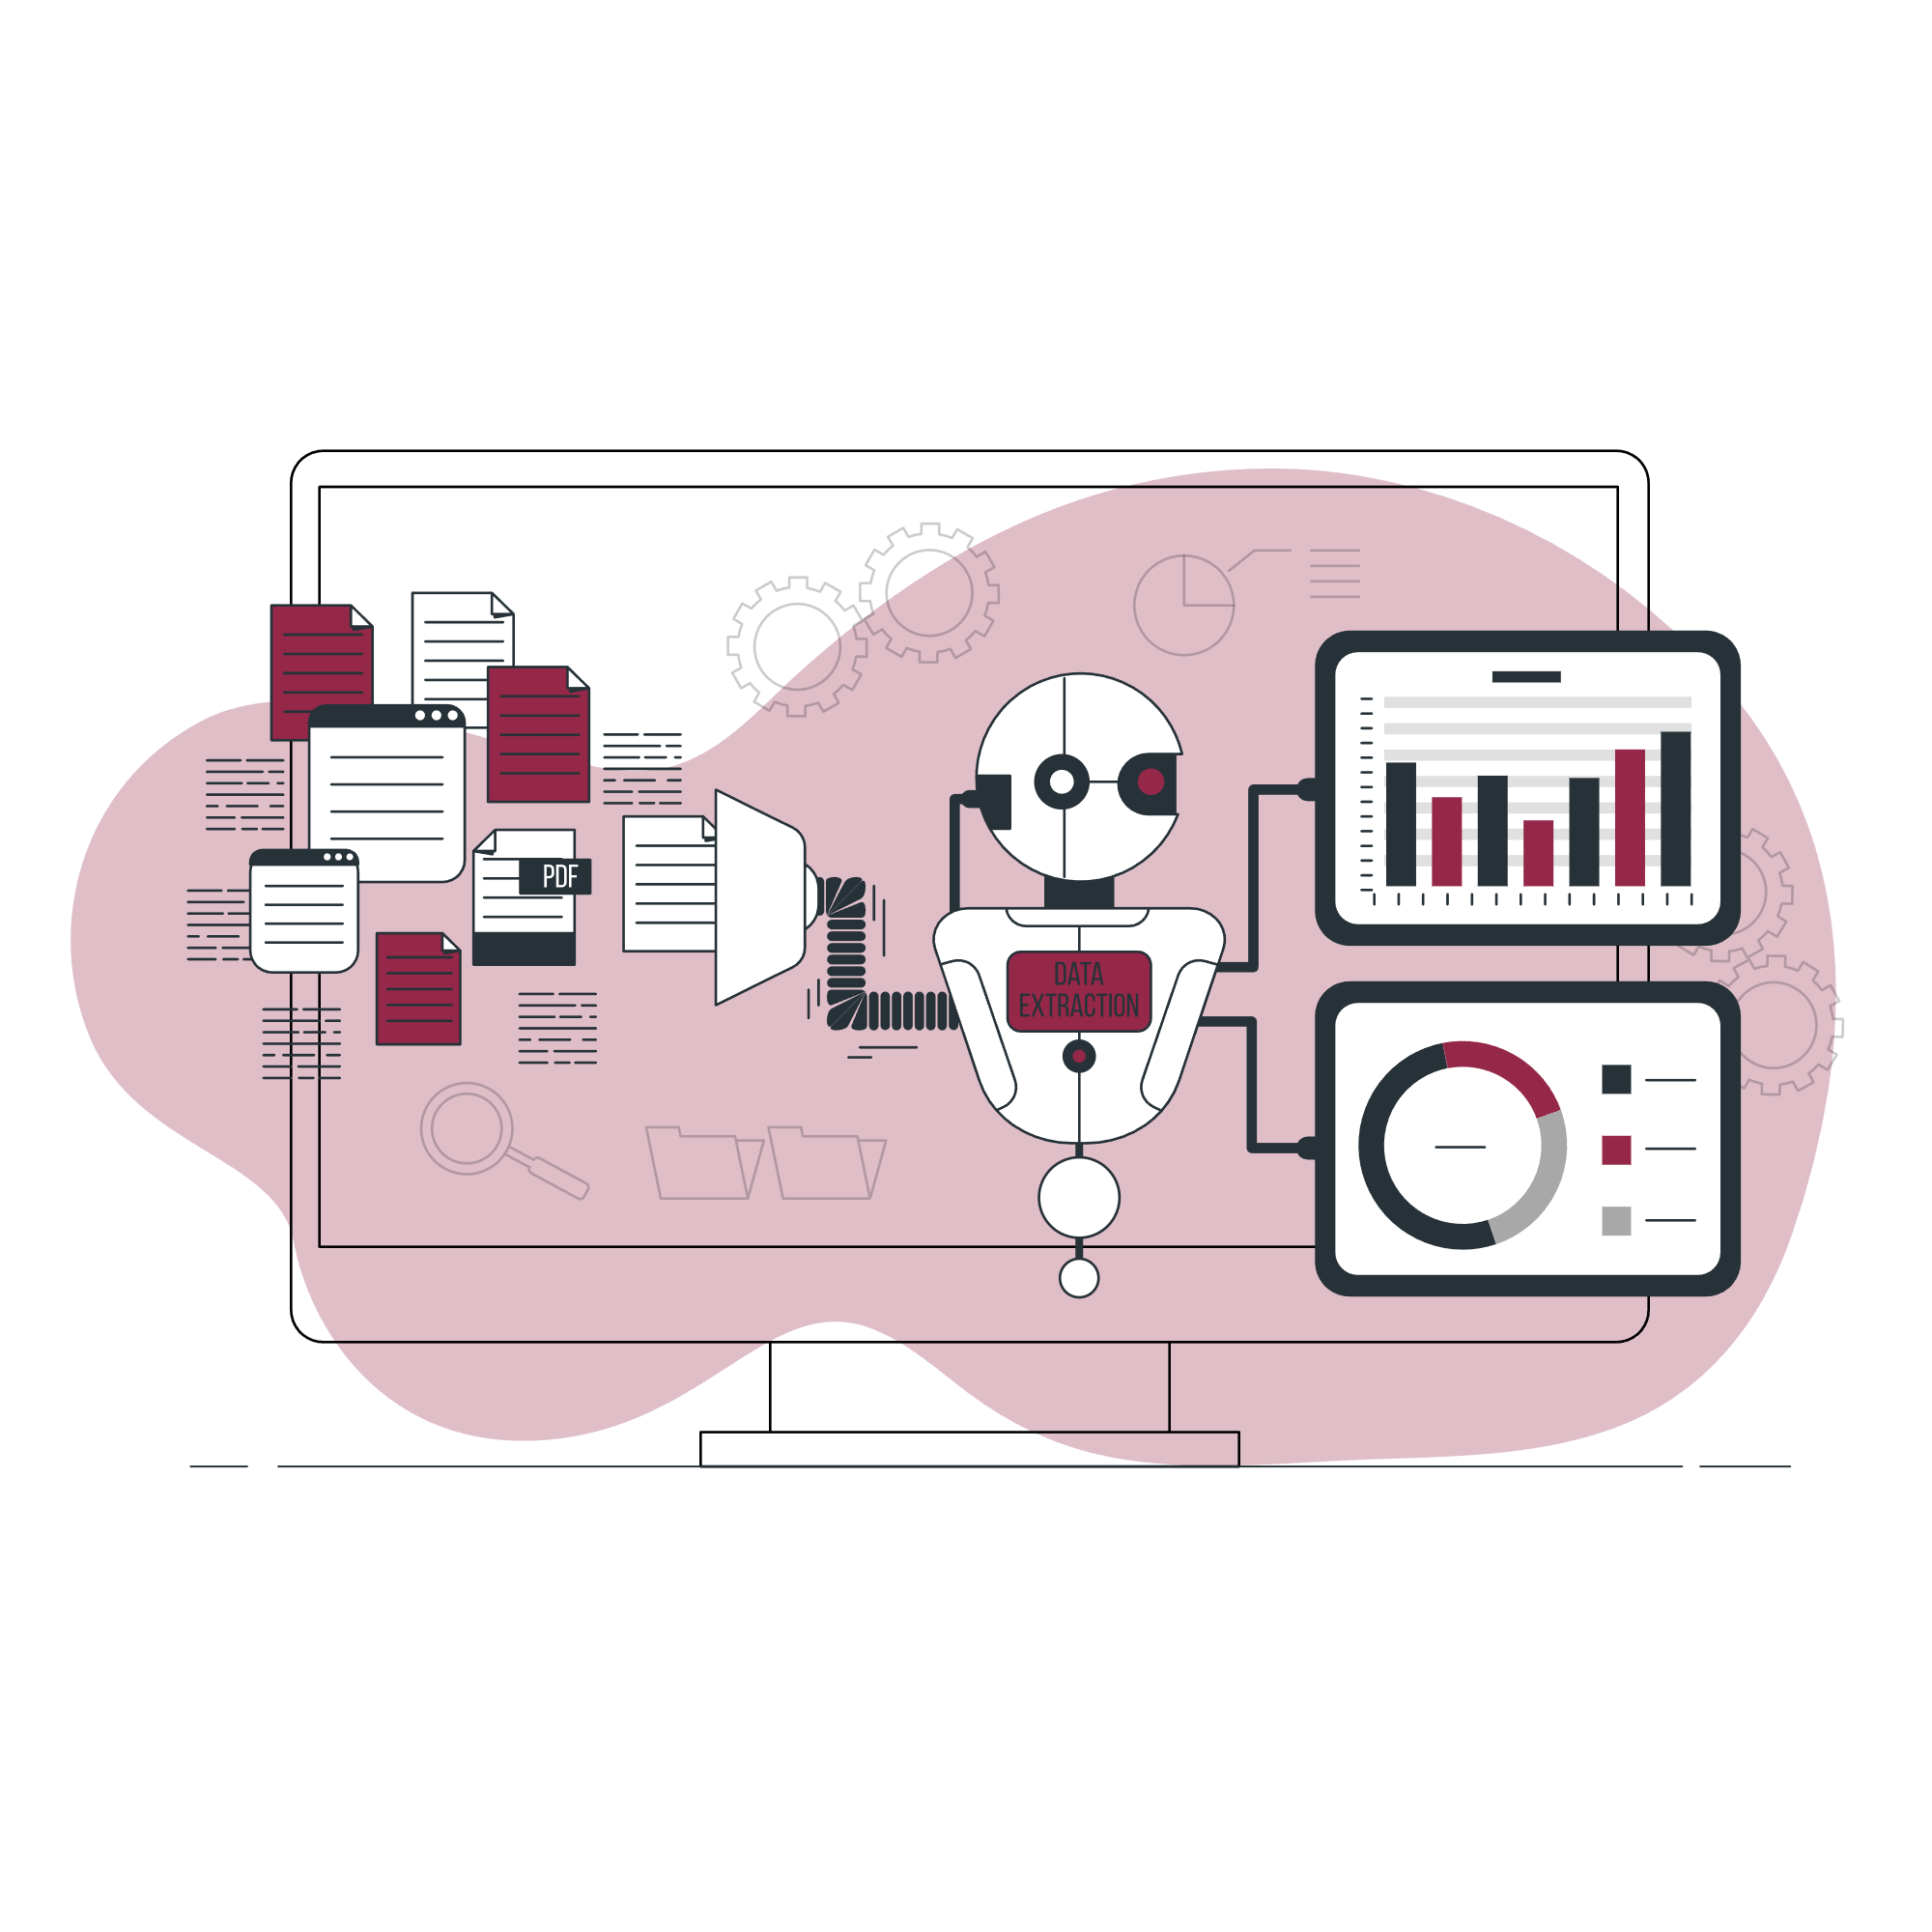
\includegraphics[width=\linewidth]{./figures/data_driven.png}
			
		\end{column}
\end{columns}

 \justifying
How can data-driven models effectively identify mental disorders in students? \cite{DEHGHANBONARI2023100238}
	
\end{frame}
	
	
\begin{frame}{Machine Learning Models}
	\begin{columns}[T]
		\begin{column}{0.5\textwidth}
			\justifying
			Machine learning models adapt to complex problems without explicit programming. They improve continuously as more data becomes available, refining predictions and staying effective in dynamic environments.
		\end{column}
		\begin{column}{0.5\textwidth}
			\centering
			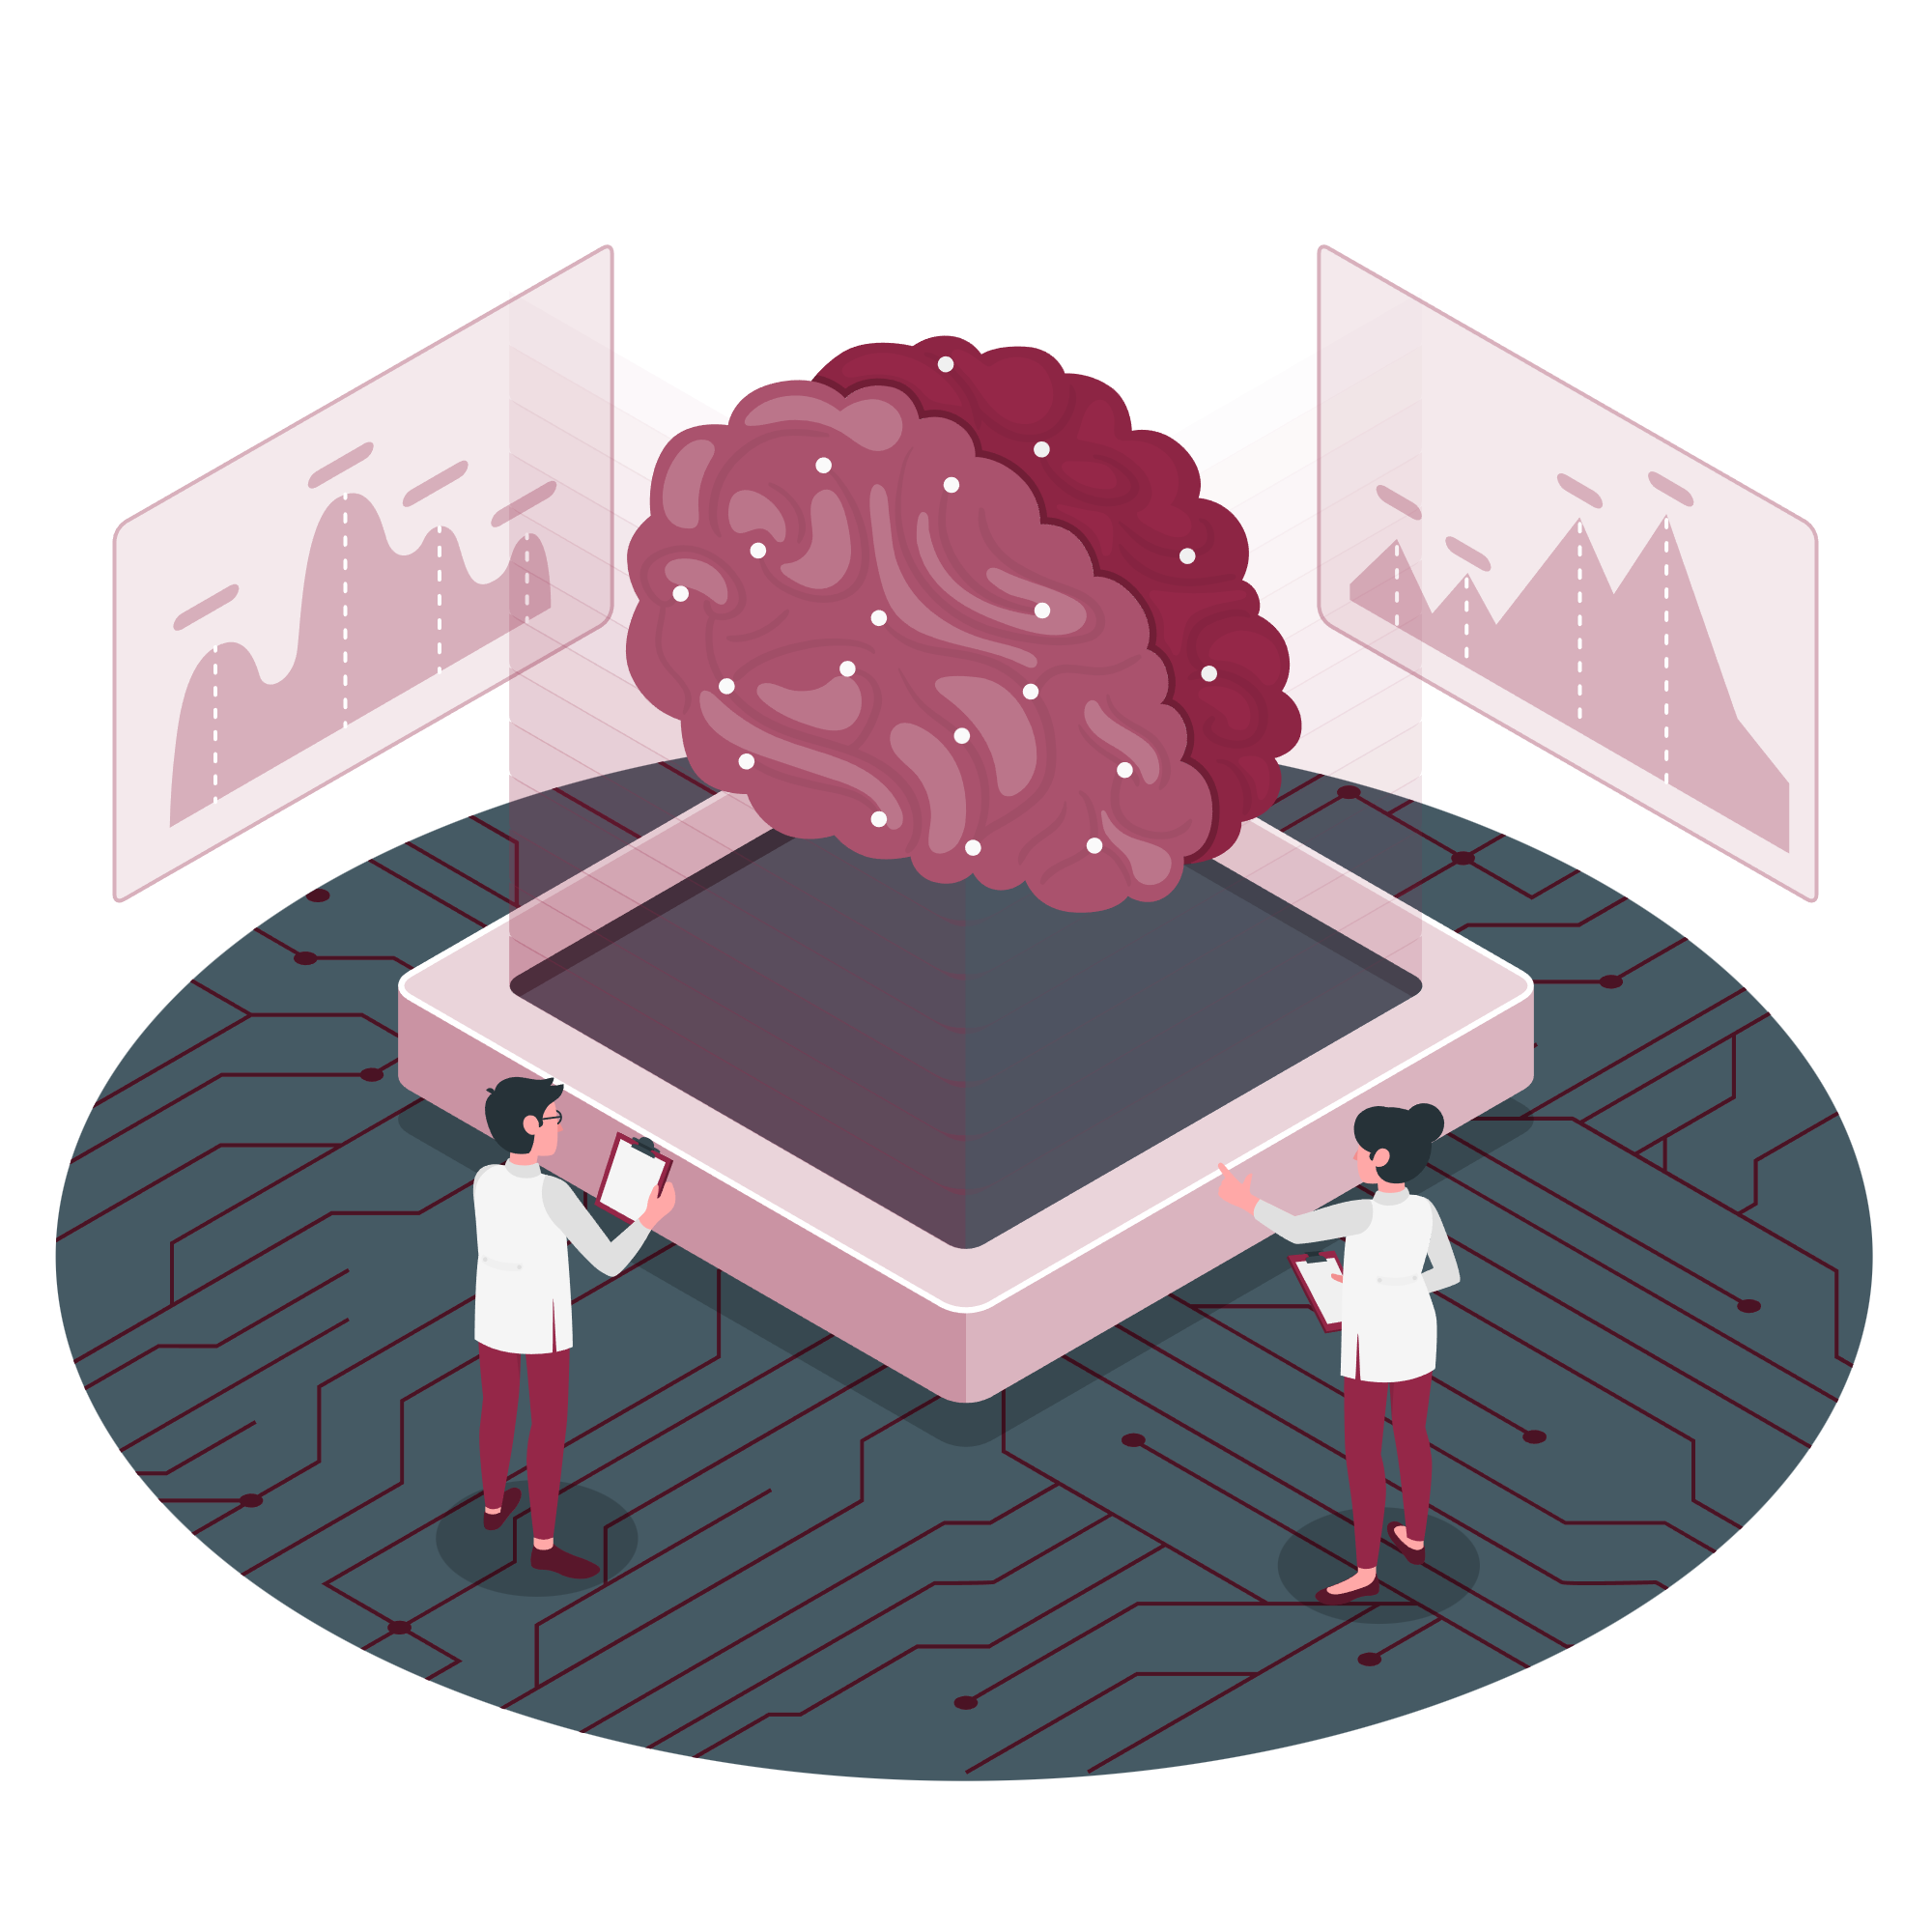
\includegraphics[width=\linewidth]{./figures/artificial_intelligence.png}
		\end{column}
	\end{columns}
\end{frame}

	

	
	
\section*{Methodology}

\begin{frame}{Three-Step Module-Based Methodology}
	
	The methodology has been divided into several steps to increase performance quality \cite{DEHGHANBONARI2023100238}.
	\vspace{0.5cm}
	
	\begin{columns}[c]
		\column{0.33\textwidth}
		\centering
		\textbf{Mental Disorder Identification} \\
		
\includegraphics[width=\linewidth]{./figures/identification.png}
		
		\column{0.33\textwidth}
		\centering
		\textbf{Student Prioritization} \\
		
\includegraphics[width=\linewidth]{./figures/priorizing.png}
		
		\column{0.33\textwidth}
		\centering
		\textbf{Therapy Scheduling} \\
		
\includegraphics[width=\linewidth]{./figures/schedule.png}
	\end{columns}
\end{frame}

	\section*{Mental Disorder Identification}
	
	\begin{frame}{Data Collection and Labeling}
		\vspace{-0.5cm}
		\begin{columns}[c]
			\column{0.5\textwidth}
			\justifying
			
			Labeled text data is used to train a machine learning model for mental disorder classification. The model classifies individuals as healthy or with mental disorders to aid diagnosis.
			
			\centering
			Input Space: \( \mathcal{X} \) (data features) \\
			Output Space: \( \mathcal{Y} = \{(l, s)\} \) \\
			\begin{itemize}
				\item \( l \): Labels
				\item \( s \): Severity level of the disorder.
			\end{itemize}
			
			\column{0.5\textwidth}
			\centering

			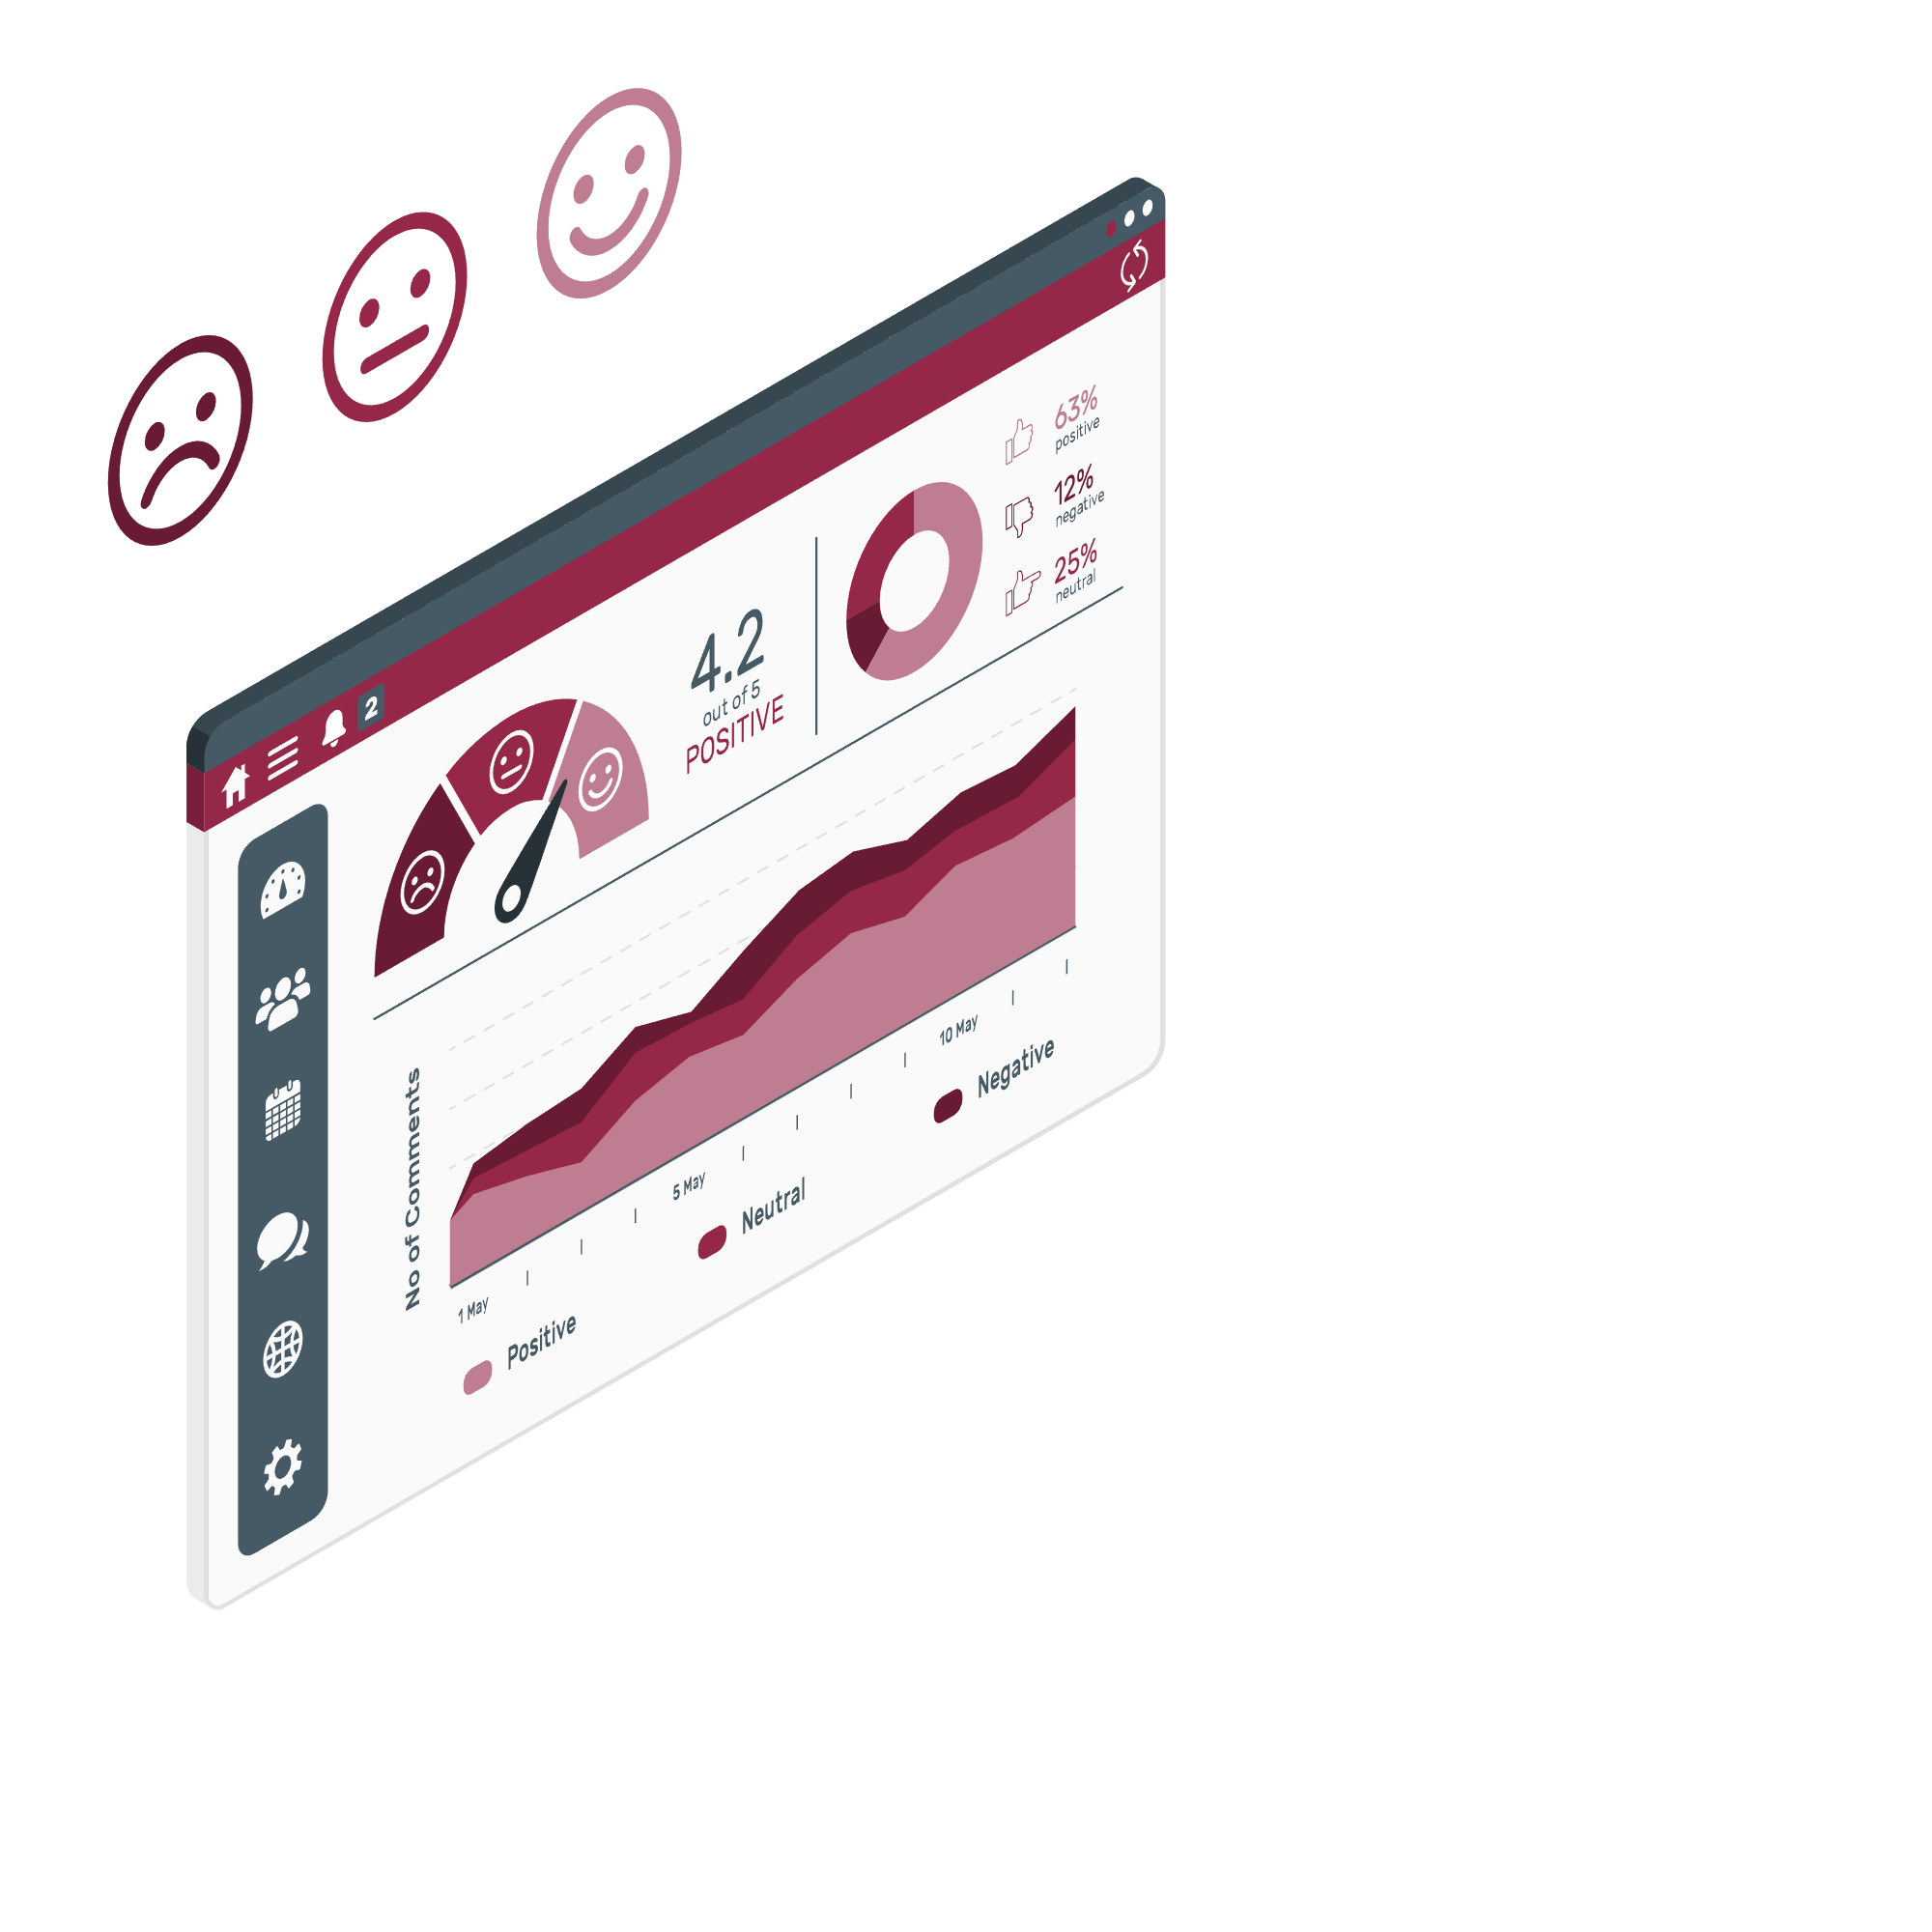
\includegraphics[width=0.8\linewidth]{./figures/sentimental_analysis.png} % Replace with your actual image path
		\end{columns}
		\vspace{0.1cm}
		\begin{columns}[c]
			\column{0.5\textwidth}
			\centering
			Data Collection \\
			\begin{tcolorbox}[width=\linewidth, colback=myNewColorB, colframe=myNewColorA, boxrule=0.7mm, rounded corners]
				\justifying
				\begin{itemize}
					\item Emails, forms, messages
					\item Course-related groups
					\item Student affairs office data
					\item Supervision by psychiatrists
				\end{itemize}
			\end{tcolorbox}
			
			\column{0.5\textwidth}
			\centering
			Data Labeling \\
			\begin{tcolorbox}[width=\linewidth, colback=myNewColorB, colframe=myNewColorA, boxrule=0.7mm, rounded corners]
				\justifying
				Expert labeling ensures reliable data for analysis, addressing cases with indirect or hard-to-measure target variables.
			\end{tcolorbox}
		\end{columns}
		
		
		
	\end{frame}
	
	
\begin{frame}{Case of Study: Mental Disorder Identification \cite{LIU2021100215}}
	
	
	\begin{tcolorbox}[width=\textwidth, colback=myNewColorB, colframe=myNewColorA, boxrule=0.7mm, rounded corners]
		This single-centre, retrospective, naturalistic study, approved by the University of Alberta Research Board, included 955 participants; 18.7\% subsequently diagnosed with Bipolar Disorder 
	\end{tcolorbox}
	
	\vspace{0.3cm}
	
	\begin{tcolorbox}[width=\textwidth, colback=myNewColorB, colframe=myNewColorA, boxrule=0.7mm, rounded corners]
		Elastic net and leave-one-out cross-validation was used to make more confident predictions at an individual level.
	\end{tcolorbox}
	
	\vspace{0.3cm}
	
	\begin{tcolorbox}[width=\textwidth, colback=myNewColorB, colframe=myNewColorA, boxrule=0.7mm, rounded corners]
		Compared to the questionnaire scoring method, the machine learning model achieved a 6.9\% improvement in accuracy.
	\end{tcolorbox}
	
\end{frame}
	
	
\section*{Student Prioritization}

\begin{frame}{Prioritization of Students for Treatment}
	
	\begin{columns}[c]
		\column{0.6\textwidth}
		\justifying
		Using the same data, a model trained on severity levels is applied. \\
		\vspace{0.3cm}
		This model prioritizes students based on the severity of their mental disorders, allowing for:
		\begin{itemize}
			\item Identification of students needing urgent psychological support.
			\item Optimization of resources by efficiently allocating psychological professionals.
			\item Ensuring timely and focused interventions for those with the highest severity levels.
		\end{itemize}
		
		\column{0.4\textwidth}
		\centering
		\vspace{-0.3cm}
		
\includegraphics[width=\linewidth]{./figures/priorizing.png}
	\end{columns}
	
\end{frame}


\begin{frame}{Case of Study: Student Prioritization \cite{https://doi.org/10.1002/jcad.12543}}
	
	
	\begin{tcolorbox}[width=\textwidth, colback=myNewColorB, colframe=myNewColorA, boxrule=0.7mm, rounded corners]
		The dataset included 61,619 students from 133 US higher education institutions and was partitioned into a 90:10 ratio for training and testing the models. 
	\end{tcolorbox}
	
	\vspace{0.3cm}
	
	\begin{tcolorbox}[width=\textwidth, colback=myNewColorB, colframe=myNewColorA, boxrule=0.7mm, rounded corners]
		They developed predictive models like, eXtreme Gradient Boosting, Random Forest, Decision Tree, and Logistic Regression to identify US college students at heightened risk of diagnosable anxiety and depressive disorders.
	\end{tcolorbox}
	
	\vspace{0.3cm}
	
	\begin{tcolorbox}[width=\textwidth, colback=myNewColorB, colframe=myNewColorA, boxrule=0.7mm, rounded corners]
		This study provides a practical tool for professional counselors to proactively identify students for anxiety and depressive disorders before these conditions escalate.
	\end{tcolorbox}
	
\end{frame}

\section*{Therapy Scheduling}

\begin{frame}{Scheduling Algorithms for Therapy Appointments}
	The action of assigning resources to perform tasks.
	\centering
	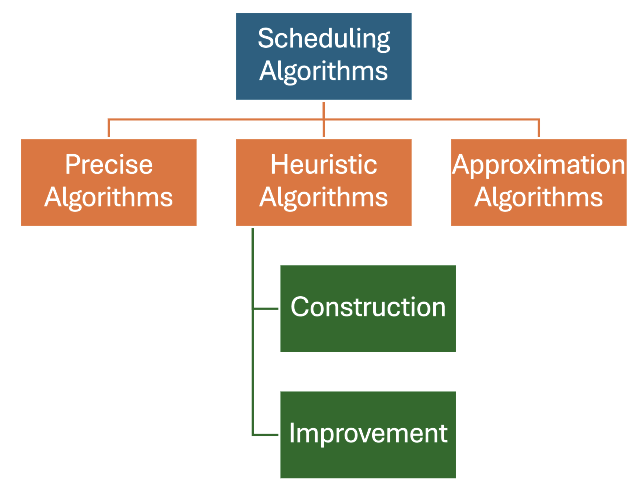
\includegraphics[width=0.65\linewidth]{./figures/scheduling_types.png} % Replace with your actual image path
	
\end{frame}

\begin{frame}{Case of Study: Therapy Scheduling \cite{DEHGHANBONARI2023100238}}
	

\begin{tcolorbox}[width=\textwidth, colback=myNewColorB, colframe=myNewColorA, boxrule=0.7mm, rounded corners]
	The collected dataset used in this case study was sourced from the renowned school in Tehran, Iran.
\end{tcolorbox}

\vspace{0.3cm}

\begin{tcolorbox}[width=\textwidth, colback=myNewColorB, colframe=myNewColorA, boxrule=0.7mm, rounded corners]
	After categorizing students and identifying high-risk groups in the current study, therapist appointments are scheduled using the Shortest Processing Time First method.
\end{tcolorbox}

\vspace{0.3cm}

\begin{tcolorbox}[width=\textwidth, colback=myNewColorB, colframe=myNewColorA, boxrule=0.7mm, rounded corners]
	By incorporating a scheduling approach, this research aimed to optimize the allocation of therapy sessions, reduce waiting times, and improve the overall service quality for students with mental disorders.
\end{tcolorbox}
	
\end{frame}
	
	
\section*{Final Remarks}

\begin{frame}{Conclusions}
	
	\begin{tcolorbox}[width=\textwidth, colback=myNewColorB, colframe=myNewColorA, boxrule=0.7mm, rounded corners]
		\begin{itemize}
			\item Extend identification accuracy of mental disorders compared to conventional methods.
			\item Prioritizes high-risk students using severity classification, optimizing therapy scheduling.
			\item Reduces waiting times and enhances access to mental health services.
			\item Supports informed decision-making by mental health professionals.
			\item Facilitates early-stage interventions, minimizing escalation of disorders.
		\end{itemize}
	\end{tcolorbox}
	
\end{frame}
	
\section*{Acknowledgments}
\begin{frame}{Acknowledgments}
	\begin{itemize}
		\item Gratitude to the Maestría en Ingeniería Eléctrica, graduate program of the Universidad Tecnológica de Pereira, for their support.
		
		\item Special thanks to ACEMATE.
		
		\item Acknowledgment to "CONVOCATORIA INTERNA PARA FINANCIACIÓN DE PROYECTOS DE ESTUDIANTES DE ESPECIALIDADES CLÍNICAS Y MAESTRÍAS AÑO 2023".
	\end{itemize}
\end{frame}

\bibliographystyle{apalike}
\bibliography{refs}

	
\end{document}

